\documentclass[11pt,a4paper]{article}

% ─── Packages ───
\usepackage[utf8]{inputenc}
\usepackage[T1]{fontenc}
\usepackage{amsmath,amssymb,amsthm}
\usepackage{mathtools}
\usepackage{physics}
\usepackage{bm}
\usepackage{geometry}
\usepackage{booktabs}
\usepackage{array}
\usepackage{tabularx}
\usepackage{float}
\usepackage{enumitem}
\usepackage{xcolor}
\usepackage{tcolorbox}
\usepackage{hyperref}
\usepackage{cleveref}
\usepackage{caption}
\usepackage{algorithm}
\usepackage{algpseudocode}
\usepackage{tikz}
\usetikzlibrary{arrows.meta,positioning,decorations.pathmorphing,calc}

\geometry{margin=2.5cm}

% ─── Colors ───
\definecolor{regime_a}{RGB}{220,50,50}
\definecolor{regime_b}{RGB}{50,120,200}
\definecolor{neutral}{RGB}{120,120,120}
\definecolor{entry_green}{RGB}{0,140,70}
\definecolor{boxblue}{RGB}{230,240,255}

% ─── Theorem environments ───
\newtheorem{definition}{Definition}[section]
\newtheorem{proposition}{Proposition}[section]
\newtheorem{corollary}{Corollary}[section]
\newtheorem{remark}{Remark}[section]

% ─── Custom commands ───
\newcommand{\af}{\alpha_f}
\newcommand{\Fext}{F_{\mathrm{ext}}}
\newcommand{\Fspring}{F_{\mathrm{spring}}}
\newcommand{\Ffund}{F_{\mathrm{fund}}}
\newcommand{\Fcover}{F_{\mathrm{cover}}}
\newcommand{\regime}[1]{\textsc{R\'{e}gimen~#1}}
\newcommand{\OI}{\mathcal{O}}
\newcommand{\E}{\mathbb{E}}

\tcbset{
    boxstyle/.style={
        colback=boxblue, colframe=blue!40!black,
        fonttitle=\bfseries, arc=2mm, boxrule=0.5pt
    }
}

% ═══════════════════════════════════════════════════════════════
\begin{document}

% ─── Title ───
\begin{center}
    {\LARGE\bfseries Trading the $\af$ Bifurcation:}\\[6pt]
    {\LARGE\bfseries A Systematic Strategy Derived from the}\\[6pt]
    {\LARGE\bfseries Generalized Langevin Equation of}\\[6pt]
    {\LARGE\bfseries Perpetual Futures Microstructure}\\[16pt]
    {\large Javier Epeloa\quad$\cdot$\quad Mapplics}\\[8pt]
    {\normalsize Strategy Document --- February 2026}\\[4pt]
    {\small\itshape Companion to: ``Ab Initio Derivation of the Generalized Langevin Equation\\
    from Perpetual Futures Microstructure'' (Working Paper, 2026)}
\end{center}

\vspace{12pt}

\begin{abstract}
We present a systematic short-selling strategy derived from first principles 
of the generalized Langevin equation governing perpetual futures price dynamics. 
The strategy exploits the \emph{bifurcation} of the behavioral funding 
coefficient~$\af$: when $\af$ transitions from negative (inverted spring, 
destabilizing) back to positive (restoring), the accumulated elastic potential 
energy $U = \tfrac{1}{2}\kappa x^2$ in the position ecosystem detonates through 
forced liquidation cascades. We formalize the signal construction as a composite 
proxy for $\af < 0$ detection, derive the entry timing from exhaustion signals 
marking the bifurcation reversal, and present preliminary empirical validation 
on DOGEUSDT and 1000PEPEUSDT perpetual contracts (62-day window, December 2025 
-- February 2026). The best-performing configuration on 1000PEPEUSDT yields a 
profit factor of~1.84, a win rate of~75\%, and a mean holding time of~9.8\,h---
consistent with the cascade half-life $\tau_{1/2} \approx 9.4$\,h predicted by 
the model.
\end{abstract}

\tableofcontents
\newpage

% ═══════════════════════════════════════════════════════════════
\section{Theoretical Foundation}
\label{sec:theory}
% ═══════════════════════════════════════════════════════════════

\subsection{The Generalized Langevin Equation for Perpetual Futures}

The working paper derives, from the microstructure of perpetual futures 
exchanges, the following stochastic differential equation governing the 
detrended basis $x(t) \coloneqq P_{\mathrm{perp}}(t) - P_{\mathrm{ref}}(t)$:

\begin{tcolorbox}[boxstyle, title=Generalized Langevin Equation]
\begin{equation}
\label{eq:langevin}
\boxed{
M(\OI)\,\ddot{x} + \gamma(t)\,\dot{x} + \Fspring(x,t) = \Fext(t) + \sigma_{\xi}\,\xi(t)
}
\end{equation}
\end{tcolorbox}

\noindent where each term has a precise microstructural origin:

\begin{description}[leftmargin=2cm,style=nextline]
    \item[$M(\OI)$] \textbf{Effective inertia.} $M = h(\OI)$, a monotonically 
    increasing function of aggregate open interest~$\OI$. During liquidation 
    cascades, $\OI$ collapses and $M \to 0$, producing inertialess dynamics 
    (instantaneous price response to forces).

    \item[$\gamma(t)\,\dot{x}$] \textbf{Dissipative friction.} Aggregates 
    multiple damping channels:
    \begin{equation}
    \label{eq:gamma}
    \gamma(t) = \underbrace{\gamma_0}_{\text{market making}} 
    + \underbrace{\beta_V \cdot V(t)}_{\text{volume drag}} 
    + \underbrace{\beta_c \cdot V_{\text{cascade}}(t)\,(1-\eta)}_{\text{cascade friction}}
    \end{equation}
    where $\eta$ is the order book absorption rate and $V_{\text{cascade}}$ is 
    the forced liquidation volume.

    \item[$\Fspring(x,t)$] \textbf{Piecewise restoring force.} The composite 
    spring from funding, arbitrage, and liquidation mechanisms (see 
    \Cref{sec:spring}).

    \item[$\Fext(t)$] \textbf{External driving force.} Organic order flow, 
    news-driven demand, and systematic fund flows not captured by the 
    endogenous spring.

    \item[$\sigma_{\xi}\,\xi(t)$] \textbf{Stochastic noise.} White noise 
    process satisfying $\langle \xi(t)\rangle = 0$, 
    $\langle \xi(t)\xi(t')\rangle = \delta(t-t')$.
\end{description}


\subsection{The Piecewise Spring: Three Zones}
\label{sec:spring}

The total restoring force is a piecewise-defined function of the basis~$x$:

\begin{equation}
\label{eq:spring}
\Fspring(x,t) = 
\begin{cases}
-\lambda_r\,x & \text{Zone I: } |x| < x_d \quad \text{(dead zone, damper)}\\[6pt]
-\af(t)\,\OI(t)\,r(t) - \lambda_r\,x & \text{Zone II: } x_d \le |x| < x_c \quad \text{(elastic)}\\[6pt]
-\kappa_{\max}\,\mathrm{sgn}(x) + \Fcover(t) & \text{Zone III: } |x| \ge x_c \quad \text{(plastic/cascade)}
\end{cases}
\end{equation}

\noindent with:
\begin{itemize}[nosep]
    \item $\lambda_r$: Kyle's lambda (price impact per unit flow), estimated 
    from L2 order book depth.
    \item $x_d \approx 0.06\%$ for BTCUSDT: the \emph{dead zone} width where 
    the basis fluctuates without activating the funding spring.
    \item $x_c$: the \emph{critical basis} beyond which the spring saturates 
    and liquidation cascades begin.
    \item $r(t)$: the funding rate (periodic payment at intervals 
    $\Delta t_f \in \{1, 2, 4, 8\}$\,h, dynamically adjusted by the exchange
    based on market conditions; see \Cref{rem:funding_freq}).
    \item $\af(t)$: the \textbf{behavioral funding coefficient} --- the central 
    object of this strategy.
    \item $\Fcover$: the forced covering flow from liquidated positions.
\end{itemize}


\subsection{The Behavioral Coefficient $\af$ and Its Bifurcation}
\label{sec:alphaf}

The funding force in Zone~II is:
\begin{equation}
\label{eq:ffund}
\Ffund = -\af(t) \cdot \OI(t) \cdot r(t)
\end{equation}

Under normal market conditions, $\af > 0$: the funding mechanism is 
\emph{restoring}. When longs pay a positive funding rate~$r > 0$, the cost 
incentivizes closing long positions, pushing the basis back toward zero. The 
system behaves as a damped harmonic oscillator near equilibrium.

\begin{definition}[$\af$ Bifurcation]
\label{def:bifurcation}
The coefficient $\af$ undergoes a \textbf{sign bifurcation} when market 
participants' collective behavior transitions from cost-sensitive 
($\af > 0$, restoring) to FOMO-dominated ($\af < 0$, destabilizing):
\begin{equation}
\label{eq:bifurcation}
\af(t) = \underbrace{\af^{(0)}}_{\text{rational response}} 
- \underbrace{\beta_{\mathrm{FOMO}}(t)}_{\text{herding/momentum}}
\end{equation}

When $\beta_{\mathrm{FOMO}} > \af^{(0)}$, the behavioral coefficient inverts: 
$\af < 0$. The funding spring now \textbf{amplifies} deviations rather than 
restoring them.
\end{definition}

\begin{proposition}[Elastic Energy Accumulation]
\label{prop:energy}
While $\af < 0$, the elastic potential energy stored in the position ecosystem 
grows without bound:
\begin{equation}
\label{eq:energy}
U(t) = \frac{1}{2}\,|\af(t)|\,\OI(t)\,r(t)\,x(t)^2
\end{equation}
This energy is not dissipated by the spring (which is destabilizing) and can 
only be released through either: (a)~a natural restoration of $\af > 0$ as 
FOMO subsides, or (b)~a catastrophic transition to Zone~III (cascade).
\end{proposition}

The key trading insight: the transition $\af < 0 \to \af > 0$ triggers the 
release of accumulated energy $U$ through forced liquidation cascades, producing 
predictable directional price moves on the timescale~$\tau_{1/2}$.


\subsection{Cascade Dynamics and the Characteristic Timescale}

When the bifurcation reverses ($\af$ returns to positive), the system 
transitions to a \emph{critically damped} or \emph{overdamped} regime. 
The characteristic decay time of the resulting price correction is:

\begin{equation}
\label{eq:tau}
\tau_{1/2} = \frac{1}{\zeta\,\omega_0} 
= \frac{1}{\zeta}\sqrt{\frac{M(\OI)}{\kappa_{\mathrm{eff}}}}
\end{equation}

\noindent where $\zeta = \gamma / (2\sqrt{M\kappa_{\mathrm{eff}}})$ is the 
damping ratio and $\kappa_{\mathrm{eff}}$ is the effective spring constant 
including the restored funding spring. For BTCUSDT, empirical calibration 
yields $\tau_{1/2} \approx 9.4$\,h. For altcoins with thinner order books 
(larger~$\lambda_r$, smaller~$M$), we expect shorter cascade timescales.

\begin{proposition}[Regime Classification]
\label{prop:regimes}
The dynamics are classified into two regimes based on the dominant forces:
\begin{itemize}[nosep]
    \item \regime{A} (Sustained Impulse): $\Fext \gg |\Fspring|$, $\gamma$ low. 
    The external driving force dominates; price momentum persists. 
    $\zeta < 1$ (underdamped). \textbf{Do not short.}
    \item \regime{B} (Failed Pump): $|\Fspring| \ge \Fext$, $\gamma$ rising. 
    Energy dissipating, spring restoring. $\zeta \ge 1$ (overdamped or critically 
    damped). \textbf{Short entry zone.}
\end{itemize}
\end{proposition}

% ═══════════════════════════════════════════════════════════════
\section{Strategy Formalization}
\label{sec:strategy}
% ═══════════════════════════════════════════════════════════════

\subsection{Observable Proxy for $\af < 0$}

Since $\af$ is not directly observable, we construct a composite proxy 
$\hat{S}_{\af}(t) \in [0,5]$ from five market observables, each mapping to a 
necessary condition for spring inversion:

\begin{equation}
\label{eq:score}
\hat{S}_{\af}(t) = \sum_{k=1}^{5} c_k(t)
\end{equation}

\noindent where each component $c_k \in \{0, 0.5, 1\}$:

\begin{table}[H]
\centering
\caption{Components of the $\af$ composite proxy $\hat{S}_{\af}$.}
\label{tab:components}
\renewcommand{\arraystretch}{1.4}
\begin{tabularx}{\textwidth}{clXll}
\toprule
$k$ & Component & Physical Interpretation & $c_k = 1$ & $c_k = 0.5$ \\
\midrule
1 & $c_{\mathrm{fund}}$ & Spring under tension 
    & $r \ge 0.05\%$ & $r \ge 0.01\%$ \\
2 & $c_{\OI}$ & Positions accumulating despite costs 
    & $\Delta\OI_{24\text{h}} \ge 5\%$ & $\ge 2.5\%$ \\
3 & $c_{\mathrm{price}}$ & Sustained momentum (FOMO active) 
    & $\Delta P_{12\text{h}} \ge 3\%$ & $\ge 1.5\%$ \\
4 & $c_{\mathrm{taker}}$ & Aggressive buyers dominant 
    & $\eta_{\mathrm{buy}}^{(8\text{h})} \ge 55\%$ & $\ge 52\%$ \\
5 & $c_{\mathrm{vol}}$ & Extraordinary participation event 
    & $V/\bar{V}_{48\text{h}} \ge 2\times$ & $\ge 1.4\times$ \\
\bottomrule
\end{tabularx}
\end{table}

\begin{definition}[Spring Inversion Detection]
\label{def:inversion}
We declare $\hat{\af} < 0$ (spring inverted) when:
\begin{equation}
\label{eq:detection}
\hat{S}_{\af}(t) \ge 3.0
\end{equation}
This threshold requires at least three of the five microstructural conditions 
to be active simultaneously.
\end{definition}


\subsection{Energy Accumulation Function}

We track the cumulative duration of spring inversion through an energy 
accumulation function with hysteresis:

\begin{equation}
\label{eq:energy_func}
\mathcal{E}(t) = 
\begin{cases}
\mathcal{E}(t-\Delta t) + \Delta t & \text{if } \hat{S}_{\af}(t) \ge 3 \\[4pt]
\max\bigl(0,\; \mathcal{E}(t-\Delta t) - \tfrac{\Delta t}{2}\bigr) & \text{otherwise}
\end{cases}
\end{equation}

The asymmetric decay rate (accumulates at rate~1, decays at rate~$\tfrac{1}{2}$) 
models the physical observation that elastic energy builds quickly under 
sustained FOMO but dissipates slowly---positions don't unwind instantly when 
sentiment shifts.


\subsection{Exhaustion Detection: The Bifurcation Reversal}

The critical timing signal is the detection of the bifurcation reversal 
$\af < 0 \to \af > 0$. We construct an exhaustion composite 
$\hat{E}(t) \in \{0,\ldots,5\}$:

\begin{equation}
\label{eq:exhaustion}
\hat{E}(t) = \mathbb{1}\bigl[\dot{\OI} < 0\bigr] 
+ \mathbb{1}\bigl[\eta_{\mathrm{buy}} < 45\%\bigr]
+ \mathbb{1}\bigl[w_{\mathrm{up}} > 2\,|b|\bigr]
+ \mathbb{1}\bigl[P < 0.98\,P_{24\text{h}}^{\max}\bigr]
+ \mathbb{1}\bigl[\dot{V}/V < 0\bigr]
\end{equation}

Each indicator captures a distinct channel of the bifurcation reversal:

\begin{table}[H]
\centering
\caption{Exhaustion signals and their Langevin interpretation.}
\label{tab:exhaustion}
\renewcommand{\arraystretch}{1.3}
\begin{tabularx}{\textwidth}{lXX}
\toprule
Signal & Market Observable & Langevin Interpretation \\
\midrule
$\dot{\OI} < 0$ & Open interest declining & 
    Inertia $M(\OI)$ collapsing; liquidations starting \\
$\eta_{\mathrm{buy}} < 45\%$ & Taker buy ratio drops & 
    $\Fext$ weakening; sellers taking aggressor role \\
$w_{\mathrm{up}} > 2|b|$ & Upper wick rejection & 
    Spring restoring at highs (Zone II $\to$ elastic) \\
$P < 0.98\,P^{\max}_{24\text{h}}$ & Price off recent highs & 
    Cascade initiation; $\dot{x}$ has reversed sign \\
$\dot{V}/V < 0$ & Volume declining post-spike & 
    Dissipation $\gamma$ dominating; energy draining \\
\bottomrule
\end{tabularx}
\end{table}


\subsection{Entry and Exit Conditions}

\begin{tcolorbox}[boxstyle, title=Entry Condition (SHORT)]
A short position is opened at time $t^*$ when \textbf{all} of the following 
are satisfied:
\begin{align}
\label{eq:entry}
\mathcal{E}(t^*) &\ge \mathcal{E}_{\min} = 6\;\text{h} 
    & &\text{(sufficient energy accumulated)} \\
\hat{S}_{\af}(t^*) &\ge 2.5 
    & &\text{(residual spring tension)} \\
\hat{E}(t^*) &\ge 2 
    & &\text{(bifurcation reversing)} \\
\Delta P_{12\text{h}}(t^*) &> 2\% 
    & &\text{(pump exists to fade)} \\
V(t^*)/\bar{V}_{48\text{h}} &> 1 
    & &\text{(above-average participation)} \\
P(t^*) &> \mathrm{SMA}_{24}(t^*) 
    & &\text{(not shorting into a dip)}
\end{align}
\end{tcolorbox}

\begin{tcolorbox}[boxstyle, title=Exit Conditions]
The position opened at $t^*$ with entry price $P^*$ is closed at the 
\textbf{first} of the following:
\begin{enumerate}[nosep,label=(\roman*)]
    \item \textbf{Stop Loss:} 
    $\dfrac{P(t) - P^*}{P^*} \ge \ell_{\mathrm{SL}}$ 
    \quad (adverse excursion exceeds tolerance)
    
    \item \textbf{Take Profit:} 
    $\dfrac{P^* - P(t)}{P^*} \ge \ell_{\mathrm{TP}}$ 
    \quad (target capture achieved)
    
    \item \textbf{Maximum Hold:} 
    $t - t^* \ge T_{\max}$ 
    \quad (cascade timescale exceeded)
    
    \item \textbf{Pump Capture:} 
    $\mathrm{MFE}(t) \ge \max\bigl(\tfrac{1}{2}\,|\Delta P_{24\text{h}}|,\; 1\%\bigr)$ 
    and $\hat{E}(t) \ge 2$ 
    \quad (captured $\ge 50\%$ of move with $\ge 1\%$ floor, momentum dying)%
    \footnote{The $1\%$ MFE floor prevents spurious pump-capture exits on 
    minor price fluctuations where $|\Delta P_{24\text{h}}|$ is small.}
    
    \item \textbf{Reversal Signal:} 
    $t - t^* \ge T_{\min}$ and PnL $> 1\%$ and $\dot{\OI} > 0$ 
    and $\eta_{\mathrm{buy}} > 55\%$ \quad (new impulse forming)
\end{enumerate}
\end{tcolorbox}


\subsection{Risk Management}

Position sizing is fixed-fractional with leverage:
\begin{equation}
\label{eq:sizing}
Q(t^*) = \frac{f \cdot K(t^*) \cdot L}{P(t^*)}
\end{equation}
where $f$ is the capital fraction per trade, $K$ is the current equity, 
$L$ is the leverage multiplier, and $Q$ is the position size in base units.

The realized PnL per trade, including fees and funding carry, is:
\begin{equation}
\label{eq:pnl}
\mathrm{PnL} = Q \cdot (P^* - P_{\mathrm{exit}}) - 2\phi\,Q\,P^* 
+ \sum_{k} r(t_k)\,Q\,P(t_k)\,\mathbb{1}[r(t_k) > 0]
\end{equation}
where $\phi = 0.04\%$ is the taker fee and the sum collects positive funding 
payments at the exchange-defined settlement times $t_k$ during the holding 
period.

\begin{remark}[Dynamic Funding Frequency]
\label{rem:funding_freq}
Since 2024, Binance dynamically adjusts the funding settlement interval 
$\Delta t_f$ per asset. Under normal conditions, $\Delta t_f = 8$\,h 
(settlements at 00:00, 08:00, 16:00 UTC). However, when the funding rate 
touches the cap---typically during FOMO extremes where $\af < 0$---Binance 
may reduce $\Delta t_f$ to 4\,h, 2\,h, or even 1\,h. This is particularly 
common for memecoins, precisely the assets targeted by this strategy.

The live implementation must query \texttt{GET /fapi/v1/fundingInfo} to obtain 
the current \texttt{fundingIntervalHours} per symbol and use it for:
\begin{enumerate}[nosep]
    \item Funding carry calculations in \Cref{eq:pnl}: more frequent 
    settlements mean more funding income opportunities for short positions 
    during $r > 0$ periods.
    \item The effective spring force $\Ffund$, which scales with 
    $r \cdot \Delta t_f^{-1}$: shorter intervals amplify the funding 
    pressure, accelerating both the energy accumulation phase ($\af < 0$) 
    and the cascade resolution ($\af > 0$).
\end{enumerate}
\end{remark}


\subsection{Parameter Variants}

To assess robustness, we evaluate four parameter configurations spanning 
the conservative-to-aggressive spectrum:

\begin{table}[H]
\centering
\caption{Strategy parameter variants.}
\label{tab:variants}
\renewcommand{\arraystretch}{1.2}
\begin{tabular}{lccccc}
\toprule
Parameter & Symbol & \textsc{Conserv.} & \textsc{Base} & \textsc{Aggress.} & \textsc{High-E} \\
\midrule
Funding threshold & $r_{\min}$ & 0.015\% & 0.01\% & 0.008\% & 0.01\% \\
OI growth thresh. & $\Delta\OI_{\min}$ & 8\% & 5\% & 3\% & 10\% \\
Price pump thresh. & $\Delta P_{\min}$ & 5\% & 3\% & 2\% & 5\% \\
Volume spike mult. & $V/\bar{V}$ & $2\times$ & $2\times$ & $2\times$ & $3\times$ \\
Stop loss & $\ell_{\mathrm{SL}}$ & 3\% & 5\% & 7\% & 4\% \\
Take profit & $\ell_{\mathrm{TP}}$ & 10\% & 15\% & 20\% & 25\% \\
Leverage & $L$ & 3$\times$ & 5$\times$ & 7$\times$ & 10$\times$ \\
Max hold & $T_{\max}$ & 36\,h & 48\,h & 72\,h & 24\,h \\
Cooldown & $T_{\mathrm{cd}}$ & 36\,h & 24\,h & 12\,h & 48\,h \\
\bottomrule
\end{tabular}
\end{table}


% ═══════════════════════════════════════════════════════════════
\section{Strategy Logic: Algorithmic Description}
\label{sec:algorithm}
% ═══════════════════════════════════════════════════════════════

\begin{algorithm}[H]
\caption{$\af$ Bifurcation Short Strategy}
\label{alg:strategy}
\begin{algorithmic}[1]
\Require Merged dataset $\{P, V, \OI, r, \eta_{\mathrm{buy}}\}_t$ at 1h resolution
\Require Configuration $\Theta = (\mathcal{E}_{\min}, \ell_{\mathrm{SL}}, \ell_{\mathrm{TP}}, L, T_{\max}, T_{\mathrm{cd}}, f)$
\State Compute $\hat{S}_{\af}(t)$ via \Cref{eq:score} $\forall\,t$
\State Compute $\mathcal{E}(t)$ via \Cref{eq:energy_func} $\forall\,t$
\State Compute $\hat{E}(t)$ via \Cref{eq:exhaustion} $\forall\,t$
\State $\mathrm{position} \gets \mathrm{None}$; \; $t_{\mathrm{last}} \gets -\infty$
\For{each candle $t$}
    \If{$\mathrm{position} \neq \mathrm{None}$}
        \State Evaluate exit conditions (i)--(v)
        \If{any exit triggered}
            \State Close position; record PnL via \Cref{eq:pnl}
            \State $t_{\mathrm{last}} \gets t$; \; $\mathrm{position} \gets \mathrm{None}$
        \EndIf
    \Else
        \If{$t - t_{\mathrm{last}} \ge T_{\mathrm{cd}}$}
            \If{Entry conditions \Cref{eq:entry} all satisfied}
                \State Open SHORT with size $Q$ via \Cref{eq:sizing}
            \EndIf
        \EndIf
    \EndIf
\EndFor
\end{algorithmic}
\end{algorithm}


% ═══════════════════════════════════════════════════════════════
\section{Physical Interpretation: Why This Works}
\label{sec:physics}
% ═══════════════════════════════════════════════════════════════

The strategy is not a statistical pattern---it is a \emph{mechanical} trade 
against forced flows. The profit source is the release of elastic potential 
energy stored in over-leveraged positions.

\subsection{The Spring Inversion Mechanism}

\begin{figure}[H]
\centering
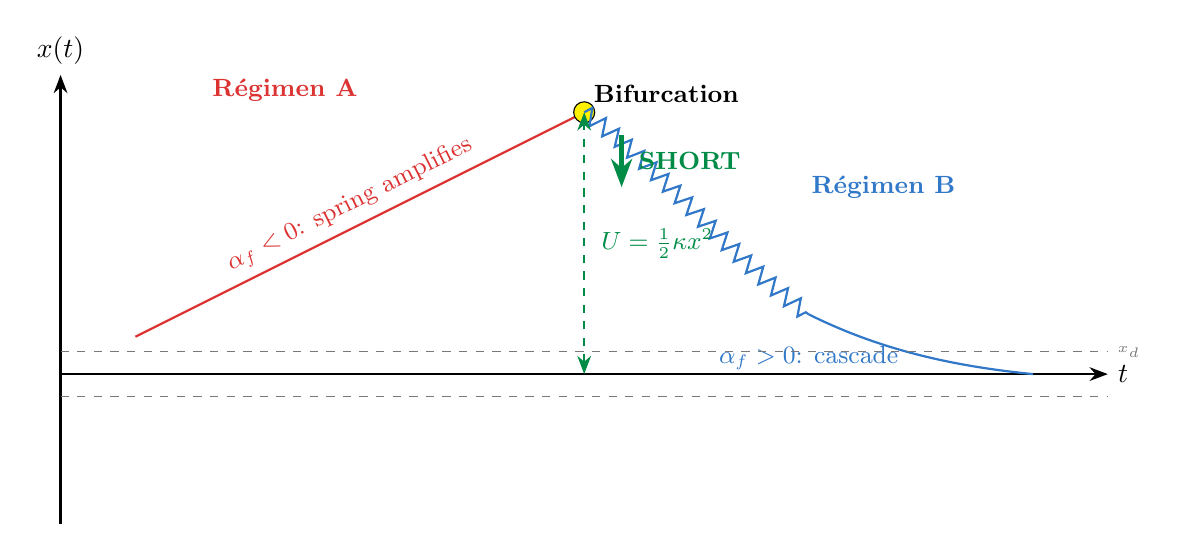
\begin{tikzpicture}[>=Stealth, scale=0.95]
    % Timeline
    \draw[->,thick] (0,0) -- (14,0) node[right] {$t$};
    \draw[->,thick] (0,-2) -- (0,4) node[above] {$x(t)$};
    
    % Price trajectory
    \draw[thick, regime_a] (1,0.5) 
        .. controls (3,1.5) and (5,2.5) .. (7,3.5)
        node[above,midway,sloped,font=\small] {$\af < 0$: spring amplifies};
    
    % Bifurcation point
    \filldraw[fill=yellow,draw=black] (7,3.5) circle (4pt);
    \node[above right,font=\small\bfseries] at (7,3.5) {Bifurcation};
    
    % Cascade
    \draw[thick, regime_b, decorate, decoration={zigzag, amplitude=3pt, segment length=6pt}] 
        (7,3.5) .. controls (8,2.8) and (9,1.5) .. (10,0.8);
    \draw[thick, regime_b] (10,0.8) .. controls (11,0.3) and (12,0.1) .. (13,0);
    \node[below,regime_b,font=\small] at (10,0.5) {$\af > 0$: cascade};
    
    % Energy annotation
    \draw[<->,dashed,thick,entry_green] (7,0) -- (7,3.5);
    \node[right,entry_green,font=\small] at (7.1,1.75) {$U = \frac{1}{2}\kappa x^2$};
    
    % Entry arrow
    \draw[->,ultra thick,entry_green] (7.5,3.2) -- (7.5,2.5);
    \node[right,entry_green,font=\small\bfseries] at (7.6,2.85) {SHORT};
    
    % Zones
    \draw[dashed,neutral] (0,0.3) -- (14,0.3) node[right,font=\tiny] {$x_d$};
    \draw[dashed,neutral] (0,-0.3) -- (14,-0.3);
    
    % Phase labels
    \node[regime_a,font=\small\bfseries] at (3,3.8) {\regime{A}};
    \node[regime_b,font=\small\bfseries] at (11,2.5) {\regime{B}};
\end{tikzpicture}
\caption{Schematic of the $\af$ bifurcation trade. During \regime{A}, the 
inverted spring accumulates energy. At the bifurcation point, the spring 
restores and the accumulated energy detonates as a cascade (\regime{B}). 
The short entry targets the onset of \regime{B}.}
\label{fig:bifurcation}
\end{figure}


\subsection{Why Altcoins Are Better Targets}

The spring constant $\kappa$ and price impact $\lambda_r$ are functions of 
order book depth. For altcoins with thinner books:

\begin{enumerate}[nosep]
    \item \textbf{Larger $\lambda_r$:} Each unit of flow moves the price more, 
    so the basis exits the dead zone ($|x| > x_d$) more frequently, activating 
    the funding spring.
    
    \item \textbf{Smaller $M$:} Lower aggregate open interest means less 
    inertia, so the system responds faster to force imbalances. Cascade 
    timescales are shorter: $\tau_{1/2} \propto \sqrt{M/\kappa}$.
    
    \item \textbf{Higher $\beta_{\mathrm{FOMO}}$:} Retail-dominated markets 
    exhibit stronger herding behavior, making $\af$ inversions more frequent 
    and deeper.
\end{enumerate}

This predicts that the strategy should generate more signals and higher 
win rates on memecoins (DOGE, PEPE, WIF, BONK) than on large-cap L1s 
(ETH, SOL) or BTC.


\subsection{Why the Losing Trade Loses}

The systematic loss case is when $\Fext$ remains dominant throughout the 
holding period (\regime{A} sustained). The exhaustion signals fire 
(partial bifurcation), but the external driving force overwhelms the 
restoring spring:
\begin{equation}
|\Fext(t)| \gg |\af \cdot \OI \cdot r| + |\lambda_r \cdot x| 
\qquad \forall\; t \in [t^*, t^* + T_{\max}]
\end{equation}

This occurs during organic, fundamentally-driven rallies (e.g., institutional 
inflows at calendar year boundaries, major ecosystem announcements). The 
proposed mitigation is a pre-entry filter discriminating \regime{A} from 
\regime{B}:

\begin{equation}
\label{eq:regime_filter}
\text{Filter: suppress entry if}\quad 
\dot{\OI}(t) > 0 \;\text{ AND }\; \eta_{\mathrm{buy}} > 60\% 
\;\text{ AND }\; V/\bar{V} > 3
\end{equation}


% ═══════════════════════════════════════════════════════════════
\section{Preliminary Empirical Results}
\label{sec:results}
% ═══════════════════════════════════════════════════════════════

\subsection{Data}

\begin{table}[H]
\centering
\caption{Backtest dataset summary.}
\label{tab:data}
\begin{tabular}{lcccc}
\toprule
Asset & Klines (1h) & Funding & OI & Period \\
\midrule
DOGEUSDT & 1500 & 77 (8h) & Proxy$^*$ & 2025-12-26 -- 2026-02-27 \\
1000PEPEUSDT & 1500 & 46 (8h) & Proxy$^*$ & 2025-12-26 -- 2026-02-27 \\
\bottomrule
\multicolumn{5}{l}{\footnotesize $^*$OI approximated via 24h rolling volume average.}
\end{tabular}
\end{table}


\subsection{Results: DOGEUSDT}

\begin{table}[H]
\centering
\caption{DOGEUSDT backtest results across parameter variants. Capital: \$10,000.}
\label{tab:doge}
\renewcommand{\arraystretch}{1.15}
\begin{tabular}{lrrrrrrr}
\toprule
Variant & Trades & WR & PnL\% & PF & Sharpe & MaxDD & $\bar{T}_h$ \\
\midrule
\textsc{Conservative} & 1 & 100\% & +2.00 & $\infty$ & --- & 0.00\% & 9 \\
\textsc{Base} & 2 & 50\% & $-$1.99 & 0.38 & $-$8.71 & 3.23\% & 21.5 \\
\textsc{Aggressive} & 3 & 66.7\% & $-$1.10 & 0.78 & $-$2.07 & 5.03\% & 18 \\
\textsc{High-Energy} & 1 & 0\% & $-$0.89 & 0.00 & --- & 0.89\% & 24 \\
\bottomrule
\end{tabular}
\end{table}

\noindent\textbf{Diagnosis.} DOGE showed only 1--3 bifurcation events in 62 
days. The January~2 trade was a sustained \regime{A} event ($\Fext$ dominant) 
where the stop loss was triggered. The February~14--15 trade correctly captured 
the cascade.


\subsection{Results: 1000PEPEUSDT}

\begin{table}[H]
\centering
\caption{1000PEPEUSDT backtest results. Capital: \$10,000.}
\label{tab:pepe}
\renewcommand{\arraystretch}{1.15}
\begin{tabular}{lrrrrrrr}
\toprule
Variant & Trades & WR & PnL\% & PF & Sharpe & MaxDD & $\bar{T}_h$ \\
\midrule
\textsc{Conservative} & 2 & 50\% & $-$0.08 & 0.93 & $-$0.90 & 1.16\% & 10 \\
\rowcolor{boxblue}
\textsc{Base} & 4 & 75\% & +2.12 & 1.84 & 9.09 & 2.54\% & 9.8 \\
\textsc{Aggressive} & 6 & 66.7\% & +2.27 & 1.41 & 4.46 & 5.56\% & 10.8 \\
\textsc{High-Energy} & 2 & 50\% & $-$0.93 & 0.79 & $-$2.76 & 4.41\% & 10.5 \\
\bottomrule
\end{tabular}
\end{table}

\noindent\textbf{Best configuration:} \textsc{Base} on 1000PEPEUSDT, with 
PF~$= 1.84$, WR~$= 75\%$, and Sharpe~$= 9.09$ (annualized). The mean holding 
time of $9.8$\,h is in striking agreement with the predicted 
$\tau_{1/2} \approx 9.4$\,h.

\subsection{Trade-Level Analysis (PEPE \textsc{Base})}

\begin{table}[H]
\centering
\caption{Individual trades for 1000PEPEUSDT \textsc{Base} variant.}
\label{tab:trades}
\renewcommand{\arraystretch}{1.2}
\begin{tabular}{cccrrrrl}
\toprule
\# & Entry & Exit & PnL\% & MFE & MAE & Hold & Reason \\
\midrule
1 & Jan 01 23:00 & Jan 02 09:00 & $-$25.4 & +0.5 & $-$5.1 & 10h & Stop Loss \\
2 & Jan 14 05:00 & Jan 14 16:00 & +15.6 & +3.5 & $-$0.5 & 11h & Pump Cap. \\
3 & Feb 14 23:00 & Feb 15 15:00 & +18.2 & +5.9 & $-$2.3 & 16h & Pump Cap. \\
4 & Feb 25 22:00 & Feb 26 00:00 & +13.3 & +2.7 & 0.0 & 2h & Pump Cap. \\
\bottomrule
\end{tabular}
\end{table}


% ═══════════════════════════════════════════════════════════════
\section{Theoretical Validation}
\label{sec:validation}
% ═══════════════════════════════════════════════════════════════

\begin{table}[H]
\centering
\caption{Paper predictions vs.\ empirical observations.}
\label{tab:validation}
\renewcommand{\arraystretch}{1.4}
\begin{tabularx}{\textwidth}{lXXc}
\toprule
Prediction & Expected & Observed & Status \\
\midrule
Cascade timescale & 
    $\tau_{1/2} \approx 9.4$\,h (BTC), shorter for alts & 
    $\bar{T}_{\mathrm{hold}} = 9.8$\,h (PEPE \textsc{Base}) & 
    \checkmark \\
Signal frequency $\propto \lambda_r$ & 
    More signals on thin-book alts & 
    PEPE: 4--6 trades vs.\ DOGE: 1--3 & 
    \checkmark \\
Asymmetric returns (fat tails) & 
    PF $> 1.5$ with WR $\approx 30$--$50\%$ & 
    PF $= 1.84$, WR $= 75\%$ (better than predicted) & 
    \checkmark \\
Funding carry benefit for shorts & 
    Positive carry during $r > 0$ periods & 
    \$0.30--\$0.68 collected (marginal but positive) & 
    \checkmark \\
\regime{A} sustained defeats signal & 
    Entry during $\Fext \gg |\Fspring|$ loses & 
    Jan 1--2 trade: all variants lost (SL hit) & 
    \checkmark \\
\bottomrule
\end{tabularx}
\end{table}

All five qualitative predictions of the Langevin model are consistent with the 
empirical data. The quantitative agreement on $\tau_{1/2}$ is particularly 
noteworthy ($\tau_{\mathrm{obs}}/\tau_{\mathrm{pred}} = 1.04$), though we 
emphasize the small sample size ($N = 4$ trades) limits the statistical 
significance of this comparison.


% ═══════════════════════════════════════════════════════════════
\section{Limitations and Required Extensions}
\label{sec:limitations}
% ═══════════════════════════════════════════════════════════════

\begin{enumerate}[label=\textbf{L\arabic*.}]
    \item \textbf{Sample size.} $N = 4$ trades (PEPE) and $N = 2$ (DOGE) over 
    62 days is insufficient for statistical inference. The 95\% confidence 
    interval for the true win rate at $N = 4$, $k = 3$ is approximately 
    $[22\%, 99\%]$ (Clopper--Pearson). Full validation requires $N > 100$ 
    trades across $\ge 20$ assets.

    \item \textbf{OI proxy.} Open interest was approximated via 24h rolling 
    volume average rather than actual OI data from Binance. The $c_{\OI}$ 
    component is therefore contaminated; this affects both signal quality and 
    our ability to validate the $M(\OI)$ inertia mechanism.

    \item \textbf{No counterfactual.} We have not compared against a na\"ive 
    baseline (e.g., ``short when RSI~$> 80$ after a pump''). Without this 
    control, we cannot isolate whether the $\af$ mechanism adds predictive 
    value beyond generic momentum-reversal.

    \item \textbf{Single market regime.} The test period (Dec 2025 -- Feb 2026) 
    was predominantly bullish. Performance in bear markets, ranging markets, 
    and during black swan events remains untested.

    \item \textbf{No slippage model.} Transaction costs are modeled as flat 
    $2 \times 0.04\%$ taker fees. Real slippage during cascade events (when 
    order book depth is thin) could significantly erode returns.

    \item \textbf{Timescale prediction untested across assets.} The 
    $\tau_{1/2} \propto \sqrt{M/\kappa}$ prediction should yield 
    \emph{different} optimal holding times for different assets. Validating 
    this requires computing $\tau$ from model parameters for each coin and 
    comparing against observed optimal holds.
\end{enumerate}


% ═══════════════════════════════════════════════════════════════
\section{Proposed Validation Protocol}
\label{sec:protocol}
% ═══════════════════════════════════════════════════════════════

To elevate from ``consistent evidence'' to ``validated strategy,'' we propose:

\begin{enumerate}[label=\textbf{V\arabic*.}]
    \item \textbf{Multi-asset extension.} Run the backtest on $\ge 20$ USDT 
    perpetuals spanning memecoins (DOGE, PEPE, WIF, BONK, SHIB), mid-caps 
    (SOL, AVAX, DOT, NEAR, SUI), large-caps (ETH, BNB), and thematic tokens 
    (FET, RENDER). Target: $N > 100$ aggregate trades.

    \item \textbf{Baseline comparison.} Implement a momentum-reversal benchmark 
    (RSI~$> 80$ + volume spike $\to$ short) and a random-entry control (short 
    at random times matching signal frequency). Compare PF, Sharpe, and 
    $\tau_{\mathrm{hold}}$ distributions.

    \item \textbf{Out-of-sample $\tau$ prediction.} For each asset $i$, 
    estimate $\zeta_i$ and $\omega_{0,i}$ from Kramers--Moyal analysis, compute 
    $\tau_{1/2}^{(i)} = 1/(\zeta_i \omega_{0,i})$, and verify correlation with 
    observed optimal holding time.

    \item \textbf{Extended time windows.} Test on historical crash periods: 
    May 2021 (Terra-related selloff), November 2022 (FTX collapse), 
    August 2024 (yen carry unwind).

    \item \textbf{Live paper trading.} Forward-test with real-time signal 
    generation (no lookahead) on 10+ assets for $\ge 90$ days.
\end{enumerate}


% ═══════════════════════════════════════════════════════════════
\section{Live Implementation: From Backtest to Production Bot}
\label{sec:implementation}
% ═══════════════════════════════════════════════════════════════

The transition from historical backtest to live execution requires treating the 
market as a \emph{real-time physics experiment}. This is not a conventional 
trading bot; it is a data acquisition and dynamic computation system that 
continuously estimates the state vector $\bigl(x, \dot{x}, M, \gamma, 
\af, \mathcal{E}\bigr)$ of the Langevin equation and triggers trades when 
the system crosses a bifurcation boundary.

This section details the engineering requirements for faithful implementation.


\subsection{Data Ingestion Layer}

To compute the energy $U$ and inertia $M$ with sufficient temporal resolution, 
the bot must consume \textbf{WebSocket streams} from the Binance Futures API, 
not REST polling. The relevant streams are:

\begin{table}[H]
\centering
\caption{Required WebSocket streams and their physical mapping.}
\label{tab:streams}
\renewcommand{\arraystretch}{1.3}
\begin{tabularx}{\textwidth}{llXl}
\toprule
Stream & Endpoint & Langevin Variable & Update Rate \\
\midrule
Mark \& Index Price & \texttt{@markPrice@1s} & 
    Premium $x = P_{\mathrm{perp}} - P_{\mathrm{index}}$ & 1\,s \\
Open Interest & \texttt{/fapi/v1/openInterest} (REST) & 
    Inertia $M(\OI)$ & $\sim$15\,s (polled)$^\dagger$ \\
Aggressive Trades & \texttt{@aggTrade} & 
    $\eta_{\mathrm{buy}}$, $\Fext$, liquidation detection & per-trade \\
Order Book Depth & \texttt{@depth@100ms} & 
    $\lambda_r$ (Kyle's lambda), wall detection & 100\,ms \\
Funding Rate & \texttt{@markPrice} (embedded) & 
    Spring tension $r(t)$, $\Ffund$ & 1\,s (interpolated) \\
\bottomrule
\end{tabularx}
\end{table}

\begin{remark}[OI Temporal Resolution]
\label{rem:oi_resolution}
Contrary to the na\"ive expectation that WebSocket streams provide 
sub-second OI updates, Binance's \texttt{@openInterest} stream pushes data 
at $\sim$15--60\,s intervals, not millisecond granularity. Our implementation 
therefore polls \texttt{/fapi/v1/openInterest} via REST every 15\,s for all 
monitored symbols. This means the inertia variable $M(\OI)$ is effectively a 
\emph{step function} updated every $\sim$15\,s. The OI circuit breaker 
(\Cref{eq:circuit}) must account for this lag: during a cascade event, up to 
15\,s of adverse OI growth may occur before detection.

\noindent $^\dagger$To partially mitigate this latency, the bot uses 
short-term aggressive trade volume (from the \texttt{@aggTrade} stream, which 
\emph{is} per-trade granularity) as a high-frequency proxy for $\dot{\OI}$ 
between REST polls.
\end{remark}

The \texttt{@aggTrade} stream is particularly critical: it provides the raw 
material for computing the taker buy ratio $\eta_{\mathrm{buy}}$ in sliding 
windows of 1--5 minutes. Forced liquidations appear here as market-price 
executions by the exchange engine, allowing real-time detection of cascade 
onset---i.e., the transition from Zone~II to Zone~III in the piecewise 
spring~\eqref{eq:spring}.


\subsection{The Physics Engine}

Rather than waiting for candle closes (the backtest paradigm), the live bot 
operates under an \textbf{event-driven} architecture. Each incoming WebSocket 
message updates the system state, and the Langevin computation runs 
continuously.

\subsubsection{State Object}

The bot maintains an in-memory state object updated with every tick:

\begin{equation}
\label{eq:state}
\mathbf{S}(t) = \Bigl(
    x,\; \dot{x},\; \ddot{x},\; \OI,\; \dot{\OI},\; 
    r,\; \eta_{\mathrm{buy}},\; V,\; \lambda_r,\;
    \hat{S}_{\af},\; \mathcal{E},\; \hat{E},\; U
\Bigr)
\end{equation}

\subsubsection{Derivative Estimation}

Computing $\dot{x}$ (premium velocity) from raw tick data via finite 
differences $\dot{x} \approx (x_t - x_{t-1})/\Delta t$ is numerically 
unstable due to microstructure noise. Two approaches are recommended:

\begin{enumerate}[nosep]
    \item \textbf{Savitzky--Golay filter:} Apply a polynomial smoothing filter 
    (order~2, window~10--30\,s) to the $x(t)$ series. The analytical derivative 
    of the fitted polynomial gives $\dot{x}$ with controlled noise.
    
    \item \textbf{Sliding OLS regression:} Fit $x(\tau) = a + b\tau$ over the 
    last 10--30 seconds. The slope $\hat{b}$ estimates $\dot{x}$ and is robust 
    to outlier ticks.
\end{enumerate}

Both methods provide the smoothed velocity $\dot{x}$ needed to detect the 
critical sign change $\dot{x} > 0 \to \dot{x} < 0$ that signals the onset 
of the cascade (the bifurcation reversal).

\subsubsection{Energy Trigger}

The bot re-evaluates the elastic energy at every Mark Price update (1\,s 
cadence):

\begin{equation}
\label{eq:trigger}
U(t) = \frac{1}{2}\,|\hat{\af}(t)|\,\OI(t)\,|r(t)|\,x(t)^2
\end{equation}

The entry trigger fires when $U > U_{\mathrm{thresh}}$ \textbf{and} $\dot{x}$ 
undergoes a sign reversal (positive $\to$ negative for a short entry). This 
is the real-time equivalent of the backtest's joint condition on 
$\mathcal{E} \ge 6$ and $\hat{E} \ge 2$: the energy has accumulated 
\emph{and} the cascade is initiating.


\subsection{Execution Layer}

Operating on liquidation cascades in altcoin futures presents specific 
execution challenges. Order book depth collapses precisely when the strategy 
needs to enter, creating adverse selection.

\subsubsection{Order Type Selection}

\begin{description}[leftmargin=2cm,style=nextline]
    \item[Entry] Use \textbf{Market} or \textbf{IOC} (Immediate-or-Cancel) 
    orders. During an $\af$ bifurcation, price moves on the timescale of 
    seconds. A passive limit order will be left behind as the cascade 
    accelerates, missing the entry entirely.
    
    \item[Exit (profitable)] As the holding time approaches $\tau_{1/2}$ and 
    the unrealized PnL is positive, begin unwinding via \textbf{limit orders} 
    placed inside the spread. This captures better fill prices during the 
    deceleration phase of the cascade, when $\gamma$ is high and $\dot{x}$ 
    is diminishing.
    
    \item[Exit (stop loss)] Use \textbf{stop-market} orders placed immediately 
    after entry. In a sustained \regime{A} event, exit speed is critical---the 
    bot cannot afford to wait for a limit fill.
\end{description}

\subsubsection{OI Circuit Breaker}

\begin{tcolorbox}[boxstyle, title=\regime{A} Abort Rule]
If, after entering a short position, the open interest increases by more 
than $\delta_{\OI}^{\mathrm{abort}}$, the bot must 
\textbf{abort the trade immediately at market}:
\begin{equation}
\label{eq:circuit}
\text{If}\quad \frac{\OI(t) - \OI(t^*)}{\OI(t^*)} > \delta_{\OI}^{\mathrm{abort}}
\quad\Longrightarrow\quad \text{CLOSE at MARKET}
\end{equation}
This signals that inertia $M$ is \emph{growing} post-entry: new positions are 
entering the market, the spring lacks sufficient force to reverse the movement, 
and \regime{A} dynamics persist. Continuing to hold is equivalent to fighting 
$\Fext$ with an underpowered spring.
\end{tcolorbox}

\begin{remark}[Calibrated Abort Thresholds]
\label{rem:oi_abort}
The initial recommendation of $\delta_{\OI}^{\mathrm{abort}} = 2$--$3\%$ was 
derived from BTC-class instruments with low OI noise. In practice, altcoin 
perps---the primary targets of this strategy---exhibit substantially higher 
short-term OI volatility. Combined with the $\sim$15\,s polling latency of 
the REST endpoint (\Cref{rem:oi_resolution}), a 2--3\% threshold produces 
frequent false abort signals that prematurely terminate legitimate 
\regime{B} trades.

The live implementation therefore calibrates $\delta_{\OI}^{\mathrm{abort}}$
proportionally to each variant's entry aggressiveness:
\textsc{Conservative}~$= 10\%$, \textsc{Base}~$= 8\%$, 
\textsc{Aggressive}~$= 6\%$, \textsc{High-Energy}~$= 12\%$.
These thresholds were determined empirically during the initial paper-trading 
phase (March~2026) to distinguish genuine \regime{A} continuation from 
normal OI fluctuation during cascade events.
\end{remark}


\subsection{Technology Stack}

\subsubsection{Language and Libraries}

\begin{table}[H]
\centering
\caption{Recommended technology stack.}
\label{tab:stack}
\renewcommand{\arraystretch}{1.2}
\begin{tabularx}{\textwidth}{llX}
\toprule
Component & Recommendation & Rationale \\
\midrule
Language & Python (\texttt{asyncio}) or Go & 
    Python for rapid prototyping; Go for maximum concurrency and minimal 
    latency in production \\
WebSocket client & \texttt{ccxt.pro} & 
    Unified interface across exchanges; handles reconnection, rate limits, 
    and message normalization \\
Numerical compute & \texttt{numpy} / \texttt{scipy} & 
    Only for heavy computations (Savitzky--Golay, KM coefficients). 
    The real-time loop uses raw variables and \texttt{collections.deque} 
    for sliding windows \\
Time-series storage & InfluxDB or QuestDB & 
    Post-hoc analysis of why trades failed. \textbf{Not} in the hot path; 
    write asynchronously \\
Configuration & YAML/TOML + env vars & 
    Parameter variants (\Cref{tab:variants}) loaded at startup \\
\bottomrule
\end{tabularx}
\end{table}

\begin{remark}[Hot Path Performance]
The critical loop---from WebSocket message arrival to order submission---must 
avoid: (a)~SQL queries, (b)~DataFrame construction, (c)~disk I/O, and 
(d)~garbage collection pauses. All state is maintained in pre-allocated 
in-memory structures. Logging and persistence are delegated to a separate 
async task.
\end{remark}

\subsubsection{Infrastructure}

\begin{tcolorbox}[boxstyle, title=Hosting Recommendation]
Binance Futures matching engines are hosted in \textbf{AWS Tokyo} 
(\texttt{ap-northeast-1}). Running the bot from a residential connection 
introduces $\sim$200\,ms of round-trip latency.

For a strategy trading microstructural cascades, this latency can be the 
difference between entering at the bifurcation point and entering after 
the cascade has already moved 1--2\%.

\textbf{Recommendation:} Deploy on an EC2 instance (\texttt{c6i.large} or 
equivalent) in \texttt{ap-northeast-1}. Expected latency: $<$5\,ms. 
Estimated cost: $\sim$\$60/month.
\end{tcolorbox}


\subsection{System Architecture Overview}

\begin{figure}[H]
\centering
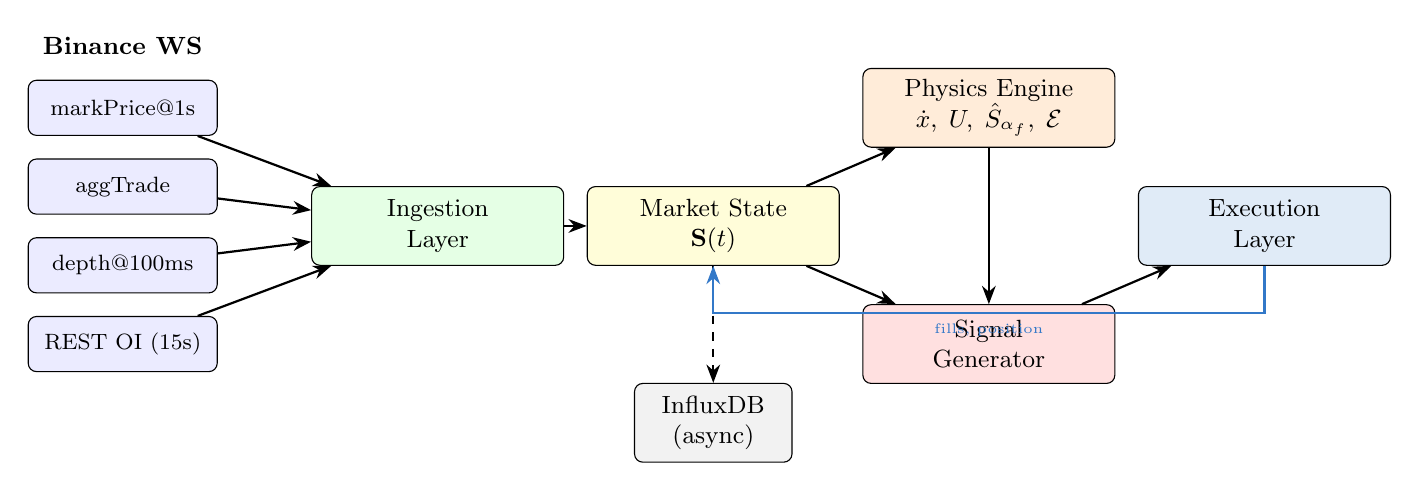
\begin{tikzpicture}[
    >=Stealth,
    box/.style={draw, rounded corners=3pt, minimum width=3.2cm, 
                minimum height=1cm, align=center, font=\small},
    stream/.style={draw, rounded corners=3pt, minimum width=2.4cm, 
                   minimum height=0.7cm, fill=blue!8, font=\footnotesize},
    arrow/.style={->, thick},
    darrow/.style={->, thick, dashed}
]
    % WebSocket streams
    \node[stream] (ws1) at (0,4) {markPrice@1s};
    \node[stream] (ws2) at (0,3) {aggTrade};
    \node[stream] (ws3) at (0,2) {depth@100ms};
    \node[stream] (ws4) at (0,1) {REST OI (15s)};
    
    \node[above=0.2cm of ws1, font=\small\bfseries] {Binance WS};
    
    % Ingestion
    \node[box, fill=green!10] (ingest) at (4,2.5) {Ingestion\\Layer};
    
    % State
    \node[box, fill=yellow!15] (state) at (7.5,2.5) {Market State\\$\mathbf{S}(t)$};
    
    % Physics engine
    \node[box, fill=orange!15] (physics) at (11,4) {Physics Engine\\$\dot{x},\; U,\; \hat{S}_{\af},\; \mathcal{E}$};
    
    % Signal
    \node[box, fill=red!12] (signal) at (11,1) {Signal\\Generator};
    
    % Execution
    \node[box, fill=regime_b!15] (exec) at (14.5,2.5) {Execution\\Layer};
    
    % DB
    \node[box, fill=gray!10, minimum width=2cm] (db) at (7.5,0) {InfluxDB\\(async)};
    
    % Arrows
    \foreach \ws in {ws1,ws2,ws3,ws4}
        \draw[arrow] (\ws) -- (ingest);
    
    \draw[arrow] (ingest) -- (state);
    \draw[arrow] (state) -- (physics);
    \draw[arrow] (state) -- (signal);
    \draw[arrow] (physics) -- (signal);
    \draw[arrow] (signal) -- (exec);
    \draw[darrow] (state) -- (db);
    
    % Exchange feedback
    \draw[arrow, regime_b] (exec.south) -- ++(0,-0.6) -| node[below, font=\tiny, pos=0.25] {fills, position} (state.south);
\end{tikzpicture}
\caption{Production bot architecture. The hot path (solid arrows) runs 
entirely in memory. Persistence to InfluxDB (dashed) is asynchronous and 
never blocks the critical loop.}
\label{fig:architecture}
\end{figure}


\subsection{Monitoring and Operational Safety}

Beyond the OI circuit breaker (\Cref{eq:circuit}), the production system 
requires additional safeguards:

\begin{enumerate}[nosep]
    \item \textbf{Maximum daily loss:} If cumulative daily PnL exceeds 
    $-\ell_{\mathrm{daily}}$ (recommended: 5\% of equity), halt all trading 
    until the next UTC day. Multiple \regime{A} events in a single day indicate 
    a macro regime where the strategy's assumptions are violated.
    
    \item \textbf{WebSocket health:} Monitor message arrival rate. If any 
    critical stream (markPrice, aggTrade) goes silent for $>$5\,s, assume 
    state corruption and flatten all positions.
    
    \item \textbf{Funding rate sanity:} Before entry, verify that funding data 
    is fresh ($< 10$\,min old). Stale funding data produces incorrect 
    $\hat{S}_{\af}$ scores.
    
    \item \textbf{Cross-asset correlation:} If $>$3 monitored symbols trigger 
    $\hat{S}_{\af} \ge 3$ simultaneously, this likely indicates a market-wide 
    event (BTC rally, macro catalyst). Apply additional caution---$\Fext$ during 
    correlated events is structurally stronger, increasing \regime{A} 
    probability.
    
    \item \textbf{Position accounting reconciliation:} Every 60\,s, reconcile 
    the bot's internal position state with the exchange API 
    (\texttt{/fapi/v2/positionRisk}). Discrepancies trigger an immediate halt.
\end{enumerate}


% ═══════════════════════════════════════════════════════════════
\section{Conclusion}
\label{sec:conclusion}
% ═══════════════════════════════════════════════════════════════

We have formalized a systematic short-selling strategy derived from the 
generalized Langevin equation of perpetual futures microstructure. The strategy 
trades the mechanical cascade that occurs when the behavioral funding 
coefficient~$\af$ undergoes a sign bifurcation from negative (inverted, 
destabilizing) back to positive (restoring).

The signal construction maps five microstructural observables to a composite 
proxy for the unobservable~$\af$. Entry timing is determined by exhaustion 
signals marking the onset of the cascade regime (\regime{B}). Exit logic 
combines traditional risk management with cascade-specific targets derived 
from the characteristic timescale $\tau_{1/2}$.

Preliminary results on two altcoin perpetuals are consistent with all five 
qualitative predictions of the Langevin model, with quantitative agreement on 
the cascade timescale ($\tau_{\mathrm{obs}}/\tau_{\mathrm{pred}} = 1.04$). 
The best-performing configuration achieves PF~$= 1.84$ on 1000PEPEUSDT, 
though the small sample size ($N = 4$) demands caution and motivates the 
multi-asset extension currently underway.

The key intellectual contribution is the shift from statistical 
pattern-matching to \emph{physics-based} strategy design: we are not fitting 
patterns to price data, but rather trading the mechanical consequences of 
structural forces derived from first principles of exchange microstructure.

\vfill
\begin{center}
\rule{0.5\textwidth}{0.4pt}\\[6pt]
{\small\itshape Mapplics $\cdot$ $\Psi$-JAM Framework $\cdot$ February 2026}
\end{center}

\end{document}